\documentclass[plainarticle,zihtitle,german,final,hyperref,utf8]{zihpub}
\usepackage{setspace}
\author{Bengt Lennicke}
\title{Komplexpraktikum "Paralleles Rechnen" \newline A - Stringmanipulationen mit Intrinsics}




\begin{document}

\section{Aufgabenstellung}

Implementieren Sie eine sequentielle und eine SIMD-parallele (mittels Intrinsics für einen Prozessor, der AVX2, AVX und FMA unterstützt) Variante für folgende String-Funktionen:
\begin{verbatim}
/* turns string "string" (with length len_string) to uppercase */
/* returns 1 if there has been an error, 0 if there has been no error */
int toUppercase(char* string, int len_string)

/* turns string "string" (with length len_string) to lowercase */
/* returns 1 if there has been an error, 0 if there has been no error */
int toLowercase(char* string, int len_string)

/* counts the appearences of character "c" in string "string" */
/* (with length len_string) */
/* returns -1 if there has been an error, and the number of appearences*/
/* if there has been no error */
int countChar(char* string, int len_string, char c)
\end{verbatim}
\begin{itemize}
	\item Beschreiben Sie für diese Funktionen die asymptotische Zeitkomplexität.
	\item Messen und Vergleichen Sie die Ausführungszeiten für sequentielle und SIMD-parallele Ausführung für Strings der Länge 10.000, 100.000, 1.000.000 und 100.000.000 .
	\item Nutzen Sie dafür die "romeo" Partition von taurus.
	\item Führen Sie jeweils 20 Messungen durch und analysieren Sie die Ergbenisse mit geeigneten statistischen Mitteln.
	
\end{itemize}

\section{Auswertung}
\subsection{Zeitkomplexität}
Die sequentiellen Funktionen für 'uppercasing', 'lowercasing' von Strings und dem Zählen von bestimmte Buchstaben in einem String sind in der Datei "string\_manipulation\_seq.c".

Die Funktionen heißen "toUppercaseSeq", "toLowercaseSeq" und "countCharSeq". Ich bin hier von den Namen der Aufgabenstellung abgewichen, damit ich den sequentiellen und paralleln Ansatz in einer Main Datei gleichzeitig importieren/nutzen kann.

Alle drei Funktionen arbeiten mit einem while loop, in welchem jedes Zeichen bearbeitet wird und anschließend der Pointer auf das nächste Zeichen bewegt wird. Damit hängt die Bearbeitungszeit linear von der Stringlänge ab. Die asymptotische Zeitkomplexität ergibt sich damit zu: O(n).
\newline

Die parallelen Funktionen sind in der Datei "string\_manipulation\_par.c" und heißen "toUppercasePar", "toLowercasePar" und "countCharPar".
Die Funktionen laden jeweils 32 Zeichen des Eingabe Strings in ein 256-bit Register. Wobei der nicht-durch-32-teilbare Rest in einen neu allokierten String geladen wird, welcher dann in das Register geladen wird. Die Funktionen zum 'uppercasing' etc. werden dann auf die jeweilingen Register angewendet.
Damit hängt die Bearbeitungszeit davon ab wie viele 32-Charakter Blöcke existieren bzw. damit von der Länge des Strings. Die asymptotische Zeitkomplexität ist also ebenfalls: O(n).
\newline

Das beschriebene Zeitverhalten ist auch in den folgenden drei Grafiken zu erkennen.
Hier wird die durchschnittlich benötigte Rechenzeit in Abhängigkeit von der Stringlänge gezeigt.
Die logarithmischen Skalen wurden gewählt, weil sonst die Messpunkte von 10k, 100k und einer Million sehr dicht zusammen liegen im Vergleich zu 100 Millionen.


\begin{figure}
	\begin{center}
		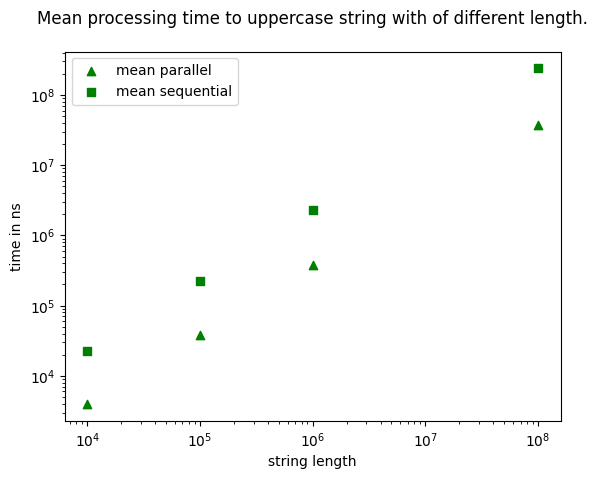
\includegraphics[width=0.7\textwidth]{images/complex_upper.png}
		\caption{Durchschnittliche Durchführungszeit von toUppercase() in Abhängigkeit von der Stringlänge.}
		\label{fig:mean_upper}
	\end{center}
\end{figure}

\begin{figure}
	\begin{center}
		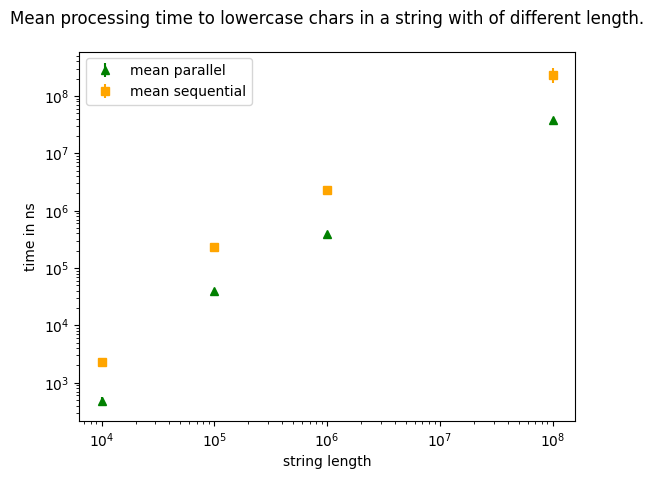
\includegraphics[width=0.7\textwidth]{images/complex_lower.png}
		\caption{Durchschnittliche Durchführungszeit von toLowercase() in Abhängigkeit von der Stringlänge.}
		\label{fig:mean_upper}
	\end{center}
\end{figure}

\begin{figure}
	\begin{center}
		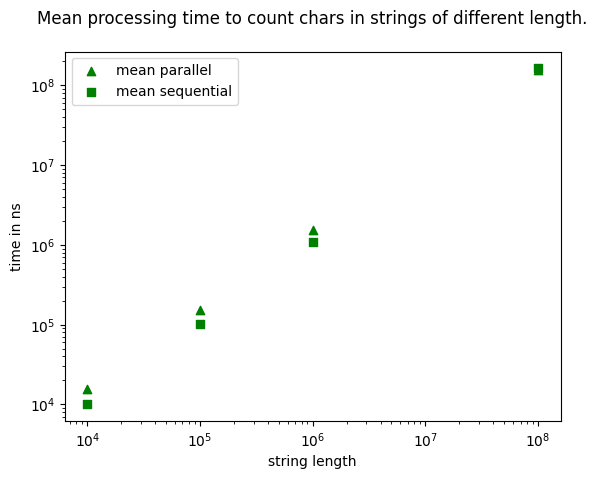
\includegraphics[width=0.7\textwidth]{images/complex_count.png}
		\caption{Durchschnittliche Durchführungszeit von countChar() in Abhängigkeit von der Stringlänge.}
		\label{fig:mean_upper}
	\end{center}
\end{figure}


\subsection{Ausführungszeiten}
\subsubsection{toUppercase}
In der Tabelle \ref{Tab:uppertab} sind die Zeitmessungen für die toUppercase() Funktionen zusammengefasst.
Es ist deutlich zu sehen, dass die sequentielle Ausführung in für jede Stringlänge mehr Zeit benötigt als die Umsetzung mit SIMD.
\newline
\begin{tabular}{|c|r|l|r|l|}
	\hline
	\multicolumn{1}{|c|}{String Länge} & \multicolumn{2}{c|}{parallel in ns} & \multicolumn{2}{c|}{sequentiell in ns} \\
	\cline{2-5}
	& Mittelwert & Standardabweichung  & Mittelwert & Standardabweichung \\
	\hline
	%\input{tabulars/lower_tab.txt} does some weird stuff and I was unable to figure out why
	10000 & 13812.89 & 2438.83 & 229699.60 & 75923.16 \\
	100000 & 74628.35 & 37815.71 & 791077.37 & 701784.15 \\
	1000000 & 781054.95 & 301556.31 & 7308699.36 & 3514745.39 \\
	100000000 & 56888725.52 & 5992509.42 & 458731319.02 & 61956346.45 \\
	\hline
\end{tabular}
\label{Tab:uppertab}


\subsubsection{toLowercase}
In der Tabelle \ref{Tab:lowertab} sind die Zeitmessungen für die toLowercase() Funktionen zusammengefasst.
Es ist deutlich zu sehen, dass die sequentielle Ausführung in für jede Stringlänge mehr Zeit benötigt als die Umsetzung mit SIMD.
\newline
\begin{tabular}{|c|r|l|r|l|}
	\hline
	\multicolumn{1}{|c|}{String Länge} & \multicolumn{2}{c|}{parallel in ns} & \multicolumn{2}{c|}{sequentiell in ns} \\
	\cline{2-5}
	& Mittelwert & Standardabweichung  & Mittelwert & Standardabweichung \\
	\hline
	%\input{tabulars/upper_tab.txt} does some weird stuff and I was unable to figure out why
	10000 & 13718.13 & 2732.00 & 311293.96 & 435716.85 \\
	100000 & 70663.97 & 33116.91 & 868215.45 & 790953.91 \\
	1000000 & 776718.16 & 328559.81 & 8446686.96 & 4419921.43 \\
	100000000 & 73948537.61 & 9256554.24 & 521830060.76 & 58353286.64 \\
	\hline
\end{tabular}
\label{Tab:lowertab}

\subsubsection{countChar}
In der Tabelle \ref{Tab:counttab} sind die Zeitmessungen für die countChar() Funktionen zusammengefasst.
Es ist zu sehen, dass die sequentielle Ausführung in für jede Stringlänge mehr Zeit benötigt als die Umsetzung mit SIMD. Hier ist der Unterschied allerdings nicht so deutlich wie bei den vorherigen Funktionen. Hier würde es sich lohnen nach einer effizienteren Lösung zu suchen als dem aktuellen Ansatz.
\newline
\begin{tabular}{|c|r|l|r|l|}
	\hline
	\multicolumn{1}{|c|}{String Länge} & \multicolumn{2}{c|}{parallel in ns} & \multicolumn{2}{c|}{sequentiell in ns} \\
	\cline{2-5}
	& Mittelwert & Standardabweichung  & Mittelwert & Standardabweichung \\
	\hline
	%\input{tabulars/count_tab.txt} does some weird stuff and I was unable to figure out why
	10000 & 46062.37 & 5738.73 & 53350.61 & 6362.82 \\
	100000 & 269818.84 & 106161.31 & 322522.16 & 122342.74 \\
	1000000 & 2617943.71 & 559510.81 & 3132603.61 & 554707.70 \\
	100000000 & 206280004.77 & 15598865.64 & 244304383.10 & 12724125.35 \\
	\hline
\end{tabular}
\label{Tab:counttab}

\newpage
\subsection{Vergleich}
In den folgenden Abbildungen sind die Laufzeiten für jeweils 100 verschiedene Strings aufgezeigt. Dabei sind pro Funktion 4 Abbildungen für je 10.000, 100.000, 1.000.000 und 100.000.000 Zeichen in den Strings. Die Diagramme veranschaulichen den Vergleich zwischen dem sequentiellen Ansatz und dem paralleln Ansatz unter Verwendung von SIMD.
\subsubsection{toUppercase}
\begin{figure}[h]
	\begin{center}
		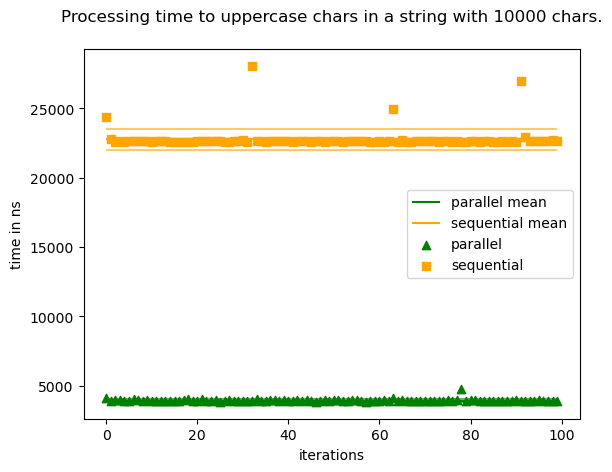
\includegraphics[width=0.65\textwidth]{images/comp_upper_10000.png}
		\caption{Durchführungszeiten von toUppercase mit 100 verschiedenen Strings mit 10.000 Zeichen.}
	\end{center}
\end{figure}
\begin{figure}[h]
\begin{center}
	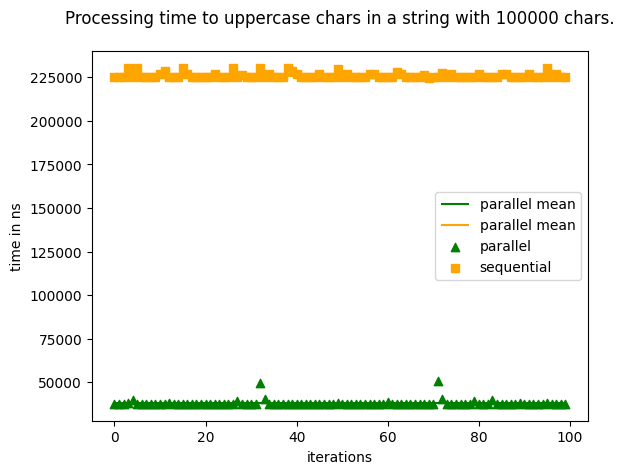
\includegraphics[width=0.65\textwidth]{images/comp_upper_100000.png}
	\caption{Durchführungszeiten von toUppercase mit 100 verschiedenen Strings mit 100.000 Zeichen.}
\end{center}
\end{figure}
\begin{figure}[h]
\begin{center}
	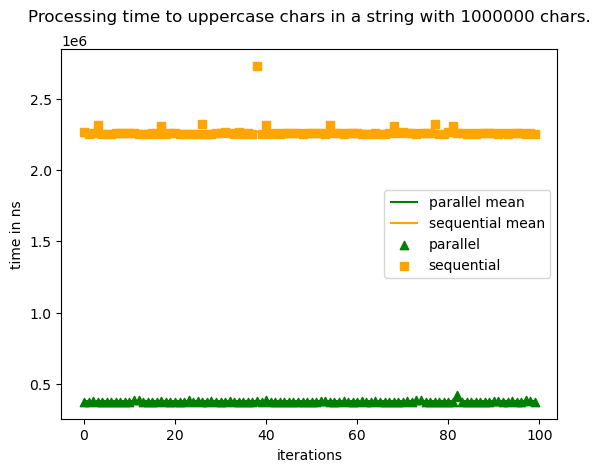
\includegraphics[width=0.65\textwidth]{images/comp_upper_1000000.png}
	\caption{Durchführungszeiten von toUppercase mit 100 verschiedenen Strings mit 1.000.000 Zeichen.}
\end{center}
\end{figure}
\begin{figure}[h]
\begin{center}
	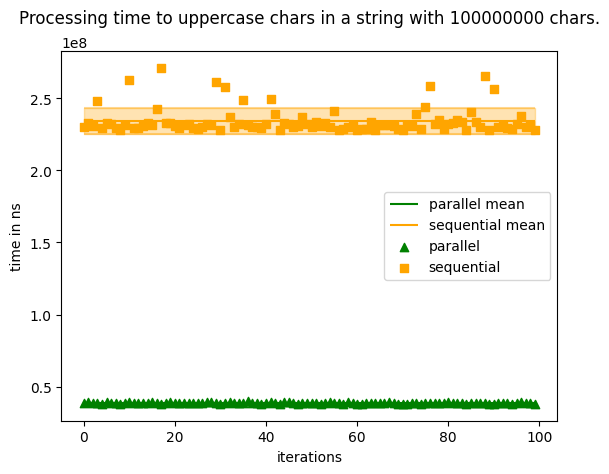
\includegraphics[width=0.65\textwidth]{images/comp_upper_100000000.png}
	\caption{Durchführungszeiten von toUppercase mit 100 verschiedenen Strings mit 100.000.000 Zeichen.}
\end{center}
\end{figure}

\clearpage
\subsubsection{toLowercase}
\begin{figure}[h]
	\begin{center}
		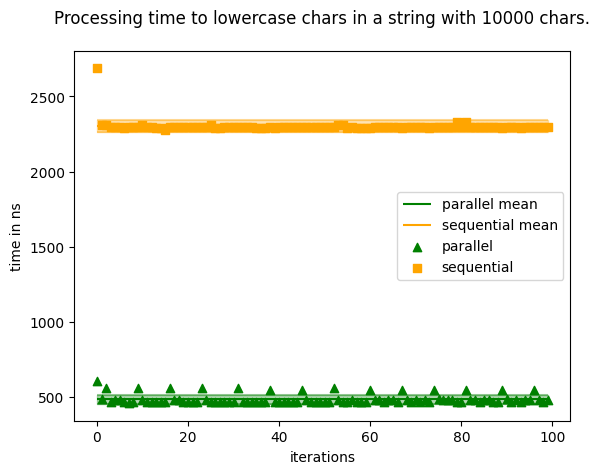
\includegraphics[width=0.65\textwidth]{images/comp_lower_10000.png}
	\end{center}
\end{figure}
\begin{figure}[h]
	\begin{center}
		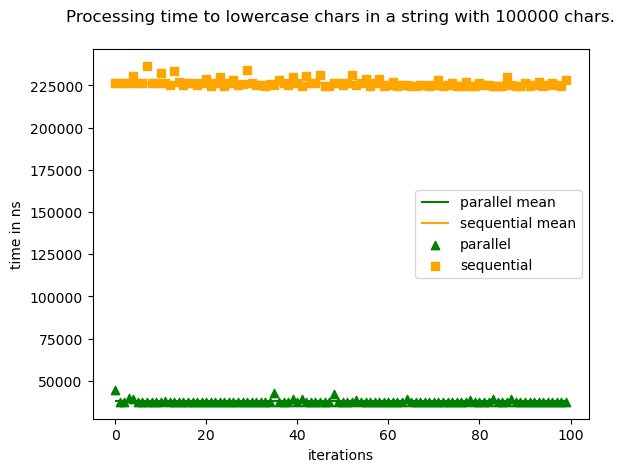
\includegraphics[width=0.65\textwidth]{images/comp_lower_100000.png}
	\end{center}
\end{figure}
\begin{figure}[h]
	\begin{center}
		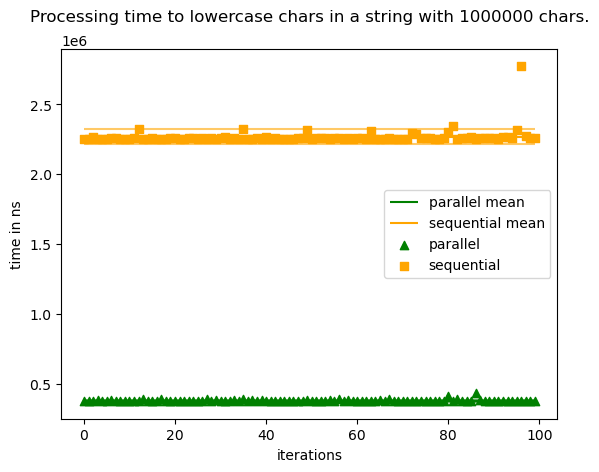
\includegraphics[width=0.65\textwidth]{images/comp_lower_1000000.png}
	\end{center}
\end{figure}
\begin{figure}[h]
	\begin{center}
		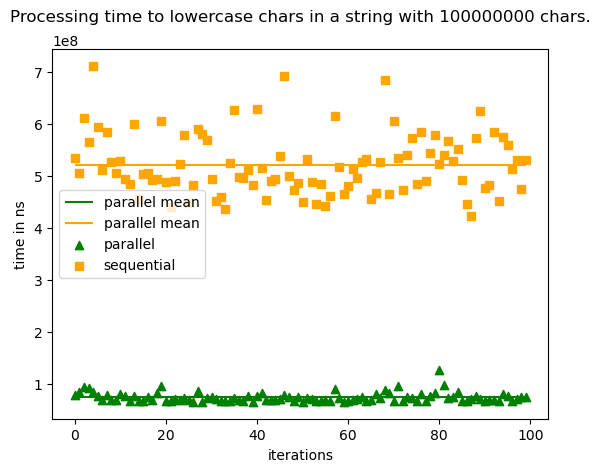
\includegraphics[width=0.65\textwidth]{images/comp_lower_100000000.png}
	\end{center}
\end{figure}

\clearpage
\subsubsection{countChar}
\begin{figure}[h]
	\begin{center}
		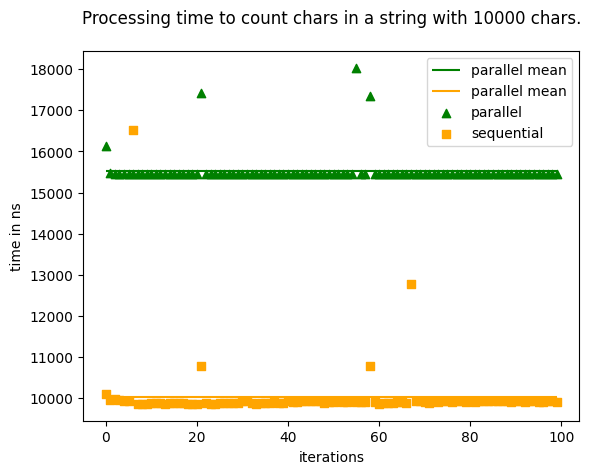
\includegraphics[width=0.65\textwidth]{images/comp_count_10000.png}
	\end{center}
\end{figure}
\begin{figure}[h]
	\begin{center}
		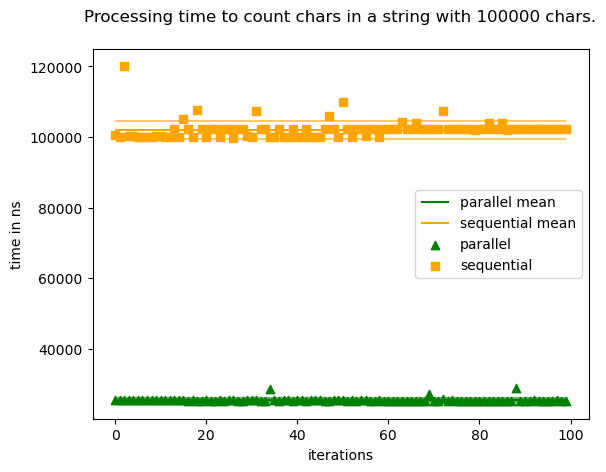
\includegraphics[width=0.65\textwidth]{images/comp_count_100000.png}
	\end{center}
\end{figure}
\begin{figure}[h]
	\begin{center}
		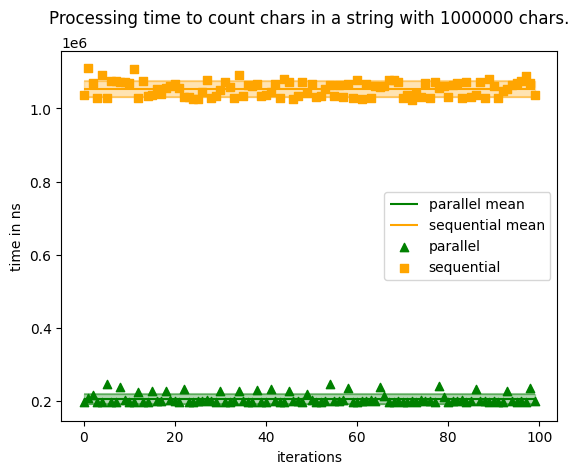
\includegraphics[width=0.65\textwidth]{images/comp_count_1000000.png}
	\end{center}
\end{figure}
\begin{figure}[h]
	\begin{center}
		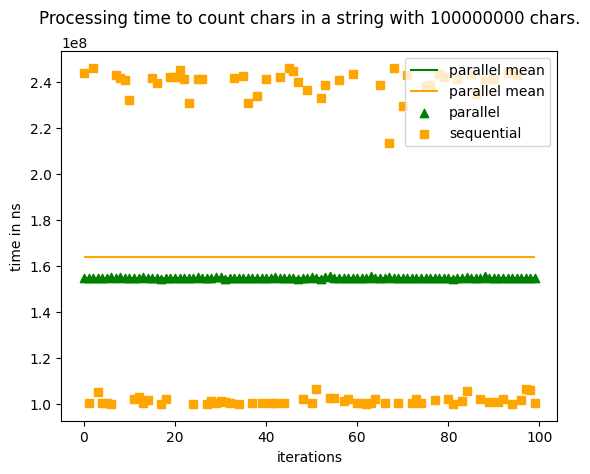
\includegraphics[width=0.65\textwidth]{images/comp_count_100000000.png}
	\end{center}
\end{figure}

\end{document}